\documentclass[10pt,a4paper]{book}
\usepackage[utf8]{inputenc}
\usepackage{amsmath}
\usepackage{amsfonts}
\usepackage{amssymb}
\usepackage{graphicx}
\begin{document}
\chapter{Transformers}
\section{Introduction to Transformers}
We often will want to understand relationships in the following pieces of data - large bodies of text, sound waves, frame-by-frame videos. The connection these data share is that they are sequential; here, there is some ordering to the pieces of data we examine. Furthermore, these features are of variable length (for example, some bodies of text or videos are longer than others).

The task at hand (the label \textbf{y}) depends. For text, we can label positive or negative sentiment analysis or label translation to another language. For audio, we can label audio transcription and speaker identification. For video, we can label and caption in-video activities. Or, they could be no label and we undergo unsupervied learning / generative modeling. 

There are several models we can use to learn from this data. There are hidden Markov / n-gram models, an array of embedding / cluster-based methods, to-be-covered-in-182 recurrent neural networks (RNNs) (gated recurrent units and long short-term memory models), convolutions (when used for sequential data, they are called "temporal convolution)", and finally, \textbf{transformers}.

Why cover transformers in this class? Well, transformers are massively influential in the field of machine learning in the last four years. They have been outcompeting other deep architectures in a number of domains, e.g., handily beating out RNNs in language modeling and convolutional networks in vision tasks. Transformers are backbone of today's famous models, BERT and GPT. With the appropriate backgroud knowledge, one can easily understand transformers.
\section{Pay Attention}
We will be borrowing from Xu et al, "Show, Attend, and Tell: Neural Image Caption Generation with Visual Attention". ICML 2015, to provide a nice example of how attention works and what it is supposed to do.

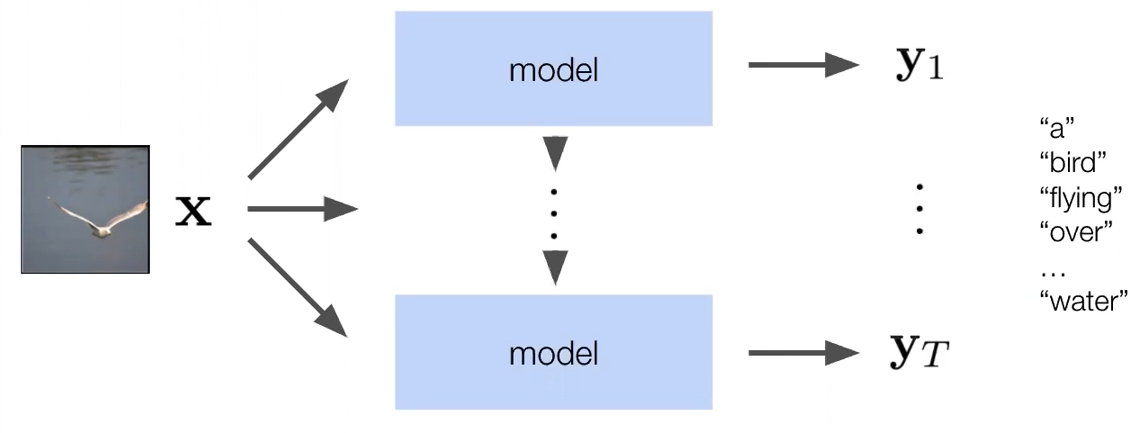
\includegraphics[width=0.8\textwidth]{images/SequentialGeneration.png}

The attention model will generate the output "one step at a time." It will repeatedly query the image to generate word after word. Somehow, the model needs to know what it has already generated in order to generate the next word. Historically, this is done using what is referred to as recurrence. 

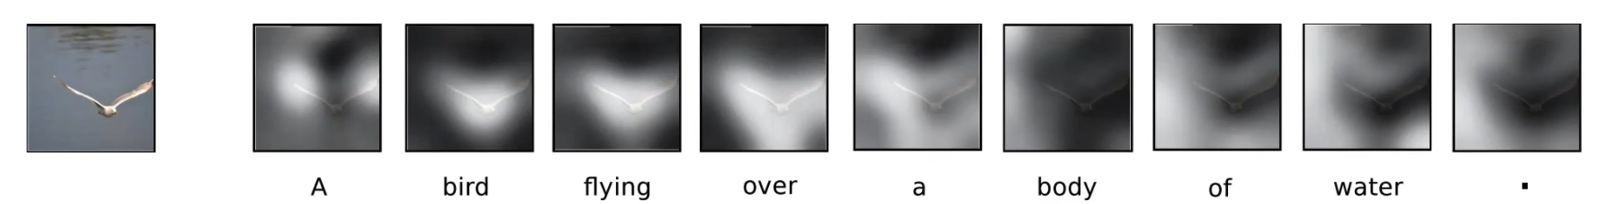
\includegraphics[width=0.9\textwidth]{images/PieceByPieceAttention.png} 

Above, we can see a visual representation of how attention will identify key features to use to sequentially output descriptive words.

\subsection{How Attention Works}
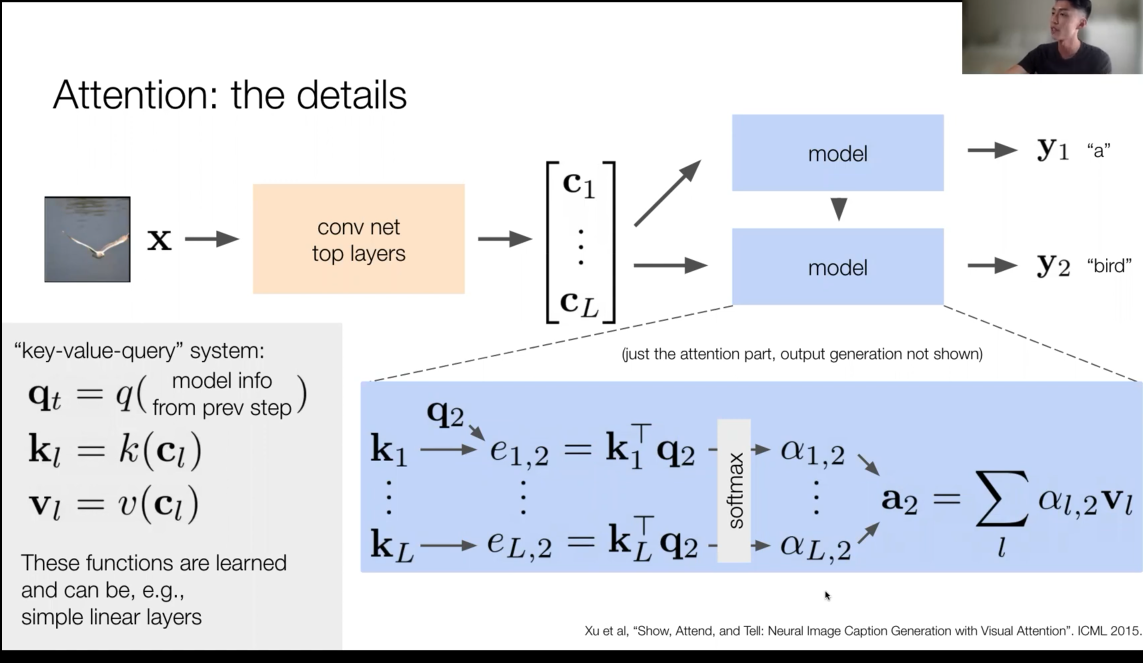
\includegraphics[width=0.9\textwidth]{images/AttentionModel.png}

In this 2015 paper, the authors developed a thorough process to generate each sequential output. First, they passed their input (in this case, an image) through the top layers of a conv net to derive high-level row-vector features that carried semantic meaning. These convolutional layers are then passed into the attention model. 

An integral piece of the attention model is the \textbf{key-value-query} system. The \textbf{queries} represent the individual pieces of output that together surmise the entire output (in image captioning, queries represent subject, article, background, descriptive words, etc.) The \textbf{keys} extract indicators about what the vectors represent (say, this vector represents the background, or that vector represents the subject), and \textbf{values} extract information corresponding to those keys (this subject is a bird, or that background is water).

For each query, we want to calculate some attention output that is close to a meaning-providing value whose corresponding key is closely associated with the piece of structure the query demands. First, we seek the right key for the query-in-question by taking the dot product (larger values indicate a greater measure of closeness) between the query vector and each key vector (for example, the first query has $k_l^T q_1$) .

We then apply this column vector of dot products to a soft-max function in order to generate a probability distribution of $\alpha$s, where the index with the highest probability corresponds to the key that most matches with the query. We then take a weighted sum and find the expectation of what the value should be.

The important qualifier is that these outputs are not final. This is just the attention part, and the ultimate output has not yet been discussed.

\textbf{In sum, each step of our attention model takes as input a matrix whose row vectors are high-level conv-net layers of the original data and returns an output that is the average of possible description-providing values, weighted by the probability matched to the level of association between the value's corresponding keys and the query in question.}

\section{Self-Attention: The Building Block of Transformers}
The goal of self-attention is to handle sequential features as the input. In some sense, self-attention is like a neural network layer that allows for processing the entire sequence all at once, rather than iterating through some time steps.
\end{document}